\documentclass[12pt]{article}
\linespread{1.3}
\usepackage{scrextend}
\usepackage{hyperref}
\usepackage{enumitem}
%\usepackage{enumerate}
\usepackage{changepage,lipsum,titlesec, longtable}
\usepackage{cite}
\usepackage{comment, xcolor}
\usepackage[pdftex]{graphicx}
  \graphicspath{{images/}, {images/stat/}}
  \DeclareGraphicsExtensions{.pdf,.jpeg,.png, .jpg}
\usepackage[cmex10]{amsmath}
\usepackage{array} 
\usepackage{subfigure} 
\usepackage{placeins} 
\usepackage{amsfonts}
\usepackage{pifont}% http://ctan.org/pkg/pifont
\usepackage{minted}

\newcommand{\cmark}{\ding{51}}%
\newcommand{\xmark}{\ding{55}}%
\newcommand{\grey}[1]{\textcolor{black!30}{#1}}
\newcommand{\red}[1]{\textcolor{red!50}{#1}}
\newcommand{\fref}[1]{Figure~\ref{#1}}
\newcommand{\tref}[1]{Table~\ref{#1}}
\newcommand{\eref}[1]{Equation~\ref{#1}}

\oddsidemargin0cm
\topmargin-2cm %I recommend adding these three lines to increase the
\textwidth16.5cm %amount of usable space on the page (and save trees)
\textheight23.5cm

\makeatletter
\renewcommand\paragraph{\@startsection{paragraph}{4}{\z@}%
            {-2.5ex\@plus -1ex \@minus -.25ex}%
            {1.25ex \@plus .25ex}%
            {\normalfont\normalsize\bfseries}}
\makeatother
\setcounter{secnumdepth}{4} % how many sectioning levels to assign numbers to
\setcounter{tocdepth}{4}    % how many sectioning levels to show in ToC

\begin{document}
\title{Building energy baseline model: next stage -- non-linear methods with rich feature set}
\maketitle
\tableofcontents
\newpage
\section{Problem specification}
\begin{itemize}
\item using a set of features to predict hourly energy
\item using a set of features to predict monthly energy we know the duration of the energy record
\item using a set of features to predict hourly energy we do not know the duration of the energy record
\end{itemize}
\section{Broad idea}
From the discussing with Professor
~\href{http://www.cs.cmu.edu/~mgormley/}{Matt Gormley}, the broad
approach should be: first create a rich feature set with all
potentially related features included, and use a non-linear model on
the rich feature set so that the training data can be nearly perfectly
predicted. Then applying some regularization to also drive down the
test error. Finally try to interpret the model by evaluating the
accuracy drop by leaving each feature out, or by incrementally adding
a feature in random order and evaluate the accuracy gain by adding
that feature.
\section{Collect input variables and representation}
A list of variables that might be important are
\begin{itemize}
\item Environmental variable
  \begin{itemize}
  \item Temperature (measured, average, or categorical): 
    \begin{itemize}
    \item outdoor air temperature
      \begin{itemize}
      \item as numerical: mean~\cite{haberl1994bin,
          hammarsten1987critical, kissock2008methodology,
          dong2005applying}, degree-day~\cite{reddy1997baselining,
          fels1986prism, pmWeather}, Radio Basis Function Kernel
        (RBFs)~\cite{wytock2013contextually},
        exact~\cite{mackay1996bayesian, Zhang2015177, cao2003support}
      \item as categorical variables~\cite{Yu20101637}
      \end{itemize}
    \item indoor air temperature~\cite{hammarsten1987critical}
    \end{itemize}
  \item Humidity
    \begin{itemize}
    \item relative humidity (RH)~\cite{dong2005applying}
    \item dew point temperature~\cite{cao2003support}
    \item exponential smoothing applied to humidity with time constant of 24h~\cite{brown2012kernel}
    \end{itemize}
  \item Solar: 
    \begin{itemize}
    \item solar radiation ($W / m^2$)~\cite{hammarsten1987critical, dong2005applying}
    \item solar flux~\cite{mackay1996bayesian}
    \item solar aperture ($m^2$)~\cite{hammarsten1987critical}, different in different time of year
    \item solar gains ($Q_S = SI, \text{unit: } W$)~\cite{hammarsten1987critical}
    \end{itemize}
  \item Wind 
    \begin{itemize}
    \item speed~\cite{mackay1996bayesian}
    \item velocity~\cite{brown2012kernel}
    \end{itemize}
  \end{itemize}
\item Occupancy
  \begin{itemize}
  \item Number of occupants~\cite{Yu20101637}
  \item Operation schedules~\cite{reddy1997baselining}
  \item Occupancy ratio (ratio of occupied vs non-occupied days)~\cite{rabl1992energy}
  \end{itemize}
\item Industry type
\item Building construction
  \begin{itemize}
  \item Detached vs apartment, categorical~\cite{Yu20101637}
  \item Construction material: wooden vs non-wooden~\cite{Yu20101637}
  \end{itemize}
\item Time
  \begin{itemize}
  \item day type (every-day, weekday, weedend)~\cite{haberl1994bin}
  \item hour of day (~\cite{haberl1994bin, wytock2013contextually},
    ~\cite{granderson2014evaluation} mean-week and
    day-time-temperature regression model)
  \item day of week (~\cite{granderson2014evaluation} mean-week, 
    day-time-temperature, and LBNL regression model)
  \item time lag ($k$), the number of previous readings to include in the model~\cite{hammarsten1987critical}
  \item unit circle representation of time of day, week, month, and year~\cite{brown2012kernel}
  \end{itemize}
\item Energy
  \begin{itemize}
  \item power ($W$, it's an auto-regressive component: use energy to
    predict energy)
    ~\cite{hammarsten1987critical}(\cite{mocanu2016deep} has some
    experiment about prediction of different time horizon using
    different time resolution)
  \item fuel type: Electric vs non-electric ~\cite{Yu20101637}
  \end{itemize}
\item Floor area~\cite{Yu20101637}
\item Building dynamics
  \begin{itemize}
  \item Heat loss coefficient ($W / m^2K$)~\cite{Yu20101637}
  \item Equivalent leakage area ($cm^2 / m^2$)~\cite{Yu20101637}
  \end{itemize}
\item Retrofit type / time
  \begin{itemize}
  \item pre-retrofit period~\cite{kissock2008methodology}
  \end{itemize}
\end{itemize}
\section{Data sources}
\subsection{Environment data sources}
In the previous stage of the work, the data source for temperature,
the only environmental variable is retrieved from the pisystem, whose
source is \href{https://www.wunderground.com/}{weather
  underground} web interface. 
\subsubsection{\href{https://gis.ncdc.noaa.gov/geoportal/catalog/search/resource/details.page?id=gov.noaa.ncdc:C00532}{Integrated Surface Global Hourly Data from NOAA}}
\begin{itemize}
\item data sample
  \begin{figure}[h!]
    \centering
    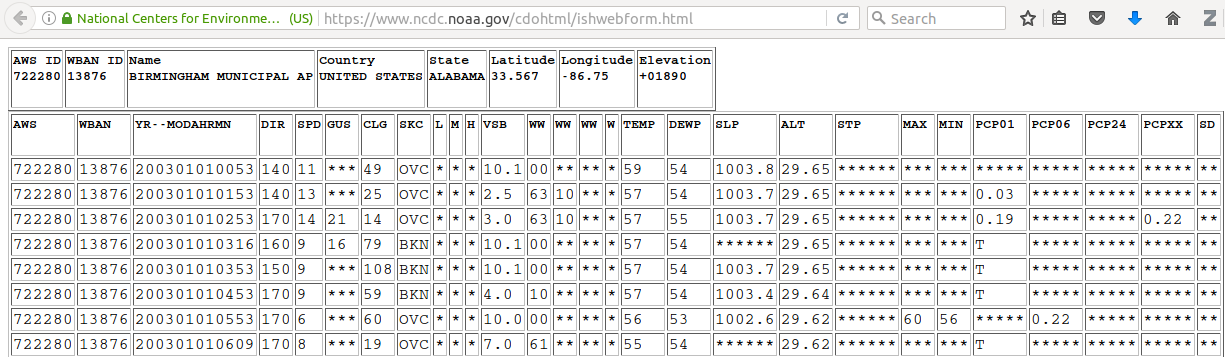
\includegraphics[width=0.8\textwidth]{images/noaa_ish.png}
    \caption{\href{https://gis.ncdc.noaa.gov/geoportal/catalog/search/resource/details.page?id=gov.noaa.ncdc:C00532}{NOAA Integrated Surface Global Hourly Data}}
    \label{fig:noaa_ish}
  \end{figure}
  \FloatBarrier
\item download: \url{ftp://ftp.ncdc.noaa.gov/pub/data/noaa/}
\item Data are ordered by year and station, each data file contains
  weather station identifier (USAF, and WBAN)
\item relevant fields: wind direction and speed, sky cover condition
  (clear, overcast, scattered, etc.), temperature, dew point,
  precipitation. 
\item time resolution: 1 to 2 observations per hour
  % token: cbacihgEFiJKKIIKJeH
% check for variables
http://www7.ncdc.noaa.gov/rest/services/variables/ish/?output=csv&token=cbacihgEFiJKKIIKJeH
% query temperature
http://www7.ncdc.noaa.gov/rest/services/values/ish/72315003812/TMP/200101010000/200101022359/?output=csv&token=cbacihgEFiJKKIIKJeH
example url: \url{https://www7.ncdc.noaa.gov/wsregistration/CDOServices.html}
\end{itemize}
\subsection{LDAS}
\section{Non-linear models}
\begin{itemize}
\item Neuron Network with 1-2 hidden layer
\item Support Vector Regression with RBF kernel
\item Random forest regression~\cite{randomForestWiki2016}
\item piecewise linear regression as baseline (it's a simple non-linear model, but not expressive enough)
\end{itemize}
\newpage
\bibliographystyle{plain}
\bibliography{myCitation}
\end{document}